\section{Scaling considerations} \label{sec:Scalings}

One important question of wall-bounded turbulence research is to find a scaling that produces a collapse of statistical quantities such as the mean velocity or the Reynolds stresses in different parts of the TBL. Ideally, the scaling parameters should include the information of the forces/boundary conditions that could affect the flow, {\it i.e.} pressure gradients, temperature gradients, friction forces, flow history, etc.
Here we have an incompressible simulation of a flat-plate turbulent boundary layer where outside of the boundary layer there is an initial zero-pressure-gradient condition, which after a certain streamwise distance evolves into an adverse-pressure-gradient condition. The scaling parameters should include the effects of the friction at the wall ($\tau_w$), the pressure gradient, the Reynolds number and the flow history.
In the literature there are many studies of self-similarity (or self-preservation) focused on the equation of momentum conservation in $x$ under some ansatz and simplifications \citep{rotta1950theorie, Townsend_1956_structure, Castillo_2004, Kitsios2016, Gibis2019}. Most of those studies find parameters that should be kept constant to achieve self-similarity. Another question regarding self-similarity is whether it can be achieved across the whole boundary layer or whether the boundary layer can only be self-similar in different regions, with various scales.


%\subsection{Self-similarity analysis and scaling of the outer region}

Following the considerations about self-similarity in \citet{Gibis2019}, two sets of scalings will be considered in the outer region for the b1.4 and ZPG databases: the edge and the Zagarola--Smits (ZS) scalings as discussed below. The equilibrium character of the boundary layer will be assessed using the Rotta--Clauser pressure-gradient parameter $\beta$ together with the pressure-gradient boundary-layer growth parameter $\Lambda_{\rm inc}$ (\ref{eq:PG_Lambda}), for the chosen outer scalings.

\begin{equation} \label{eq:PG_Lambda}
    \Lambda_{\rm inc}=\frac{L_s}{\rho U_s^2 (\mathrm{d}L_s/\mathrm{d} x)} \frac{\mathrm{d}p}{\mathrm{d}x}.
\end{equation}
In the parameter $\Lambda_{\rm inc}$, $L_s$ represents the chosen length scale and $U_s$ the velocity length scale. If $L_s=\delta^*$ and $U_s=u_{\tau}$, then the difference with respect to the parameter $\beta$ will be given by the streamwise derivative of the length scale $\textrm{d} L_s/\textrm{d}x$, which contains some information of the flow history linking the local profile with the surrounding flow.
The different scalings with their respective velocity and length scales are summarized in table \ref{tab:Scaling_parameters}.
In figure \ref{fig:pg_parameters} the pressure-gradient parameter $\Lambda_{\rm inc}$ is shown for simulation b1.4 in the first row. While the edge scaling (left) shows a monotonically rising $\Lambda_{\rm inc}$ from the beginning, the ZS scaling (right) exhibits an initial peak, then a plateau, and finally a slowly-increasing region. On the other hand, $\beta$ (figure \ref{fig:beta}) exhibits a maximum and a slow monotonic decrease throughout the domain. Recalling that the ROI starts at $\Rey_{\tau}=800$, the range of variation of the PG parameter within the ROI is $[0.2, 0.25]$ for the edge scaling, $[3.2, 4]$ for the ZS scaling and $[1.65, 1.2]$ for $\beta$. The rates of variation of the PG parameters and $\textrm{d} L_s/\textrm{d}x$ over the ROI, although not constant, are relatively small, which is a requirement for similarity according to the various studies.

%*********************************************************************************
% Tobias Gibis JFM2019  "Self-Similar compressible turbulent...outer layer."
%*********************************************************************************
\begin{table}
  \begin{center}
\def~{\hphantom{0}}
    \begin{tabular}{ l c  c  l}
    Scaling         &     $L_s$        & $U_s$                          & Reference  \\[3pt]
    Rotta--Clauser  &  $U_e^+\delta^*$ & $u_{\tau}$                     & \cite{Clauser_1956}   \\
    Edge            &  $\delta^*$      & $U_e$                          & \cite{Kitsios2016}    \\
    Zagarola--Smits &  $\delta_{99}$   & $U_{e}(\delta^*/\delta_{99})$  & \cite{zagarola_smits} \\
    \end{tabular}
  \caption{Parameters for different scalings, where $L_s$ and $U_s$ correspond to the length and velocity scales, respectively.}
  \label{tab:Scaling_parameters}
  \end{center}
\end{table}

\begin{figure}
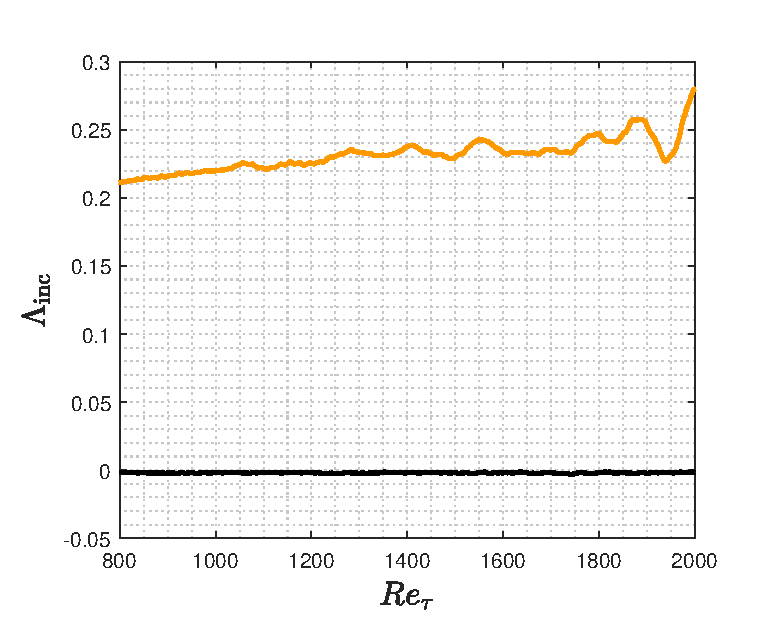
\includegraphics[width=0.49\textwidth]{fig7a.eps}
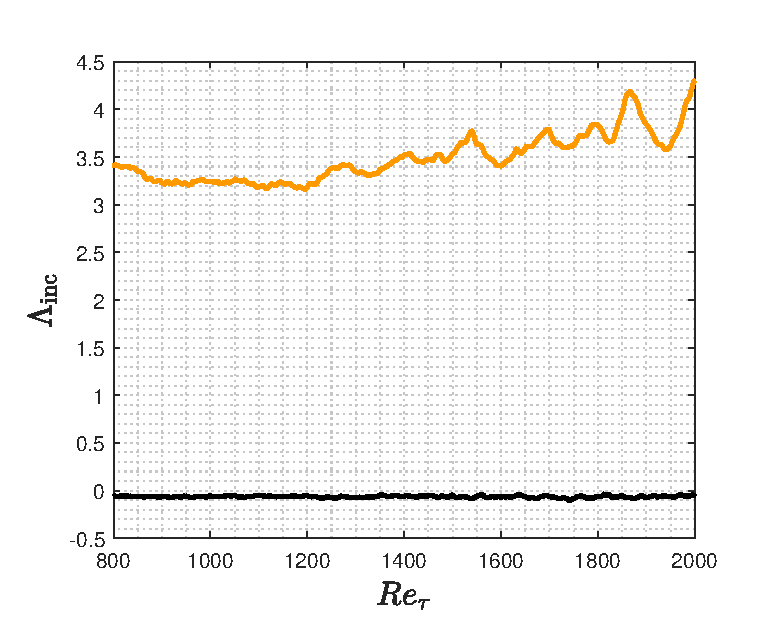
\includegraphics[width=0.49\textwidth]{fig7b.eps}
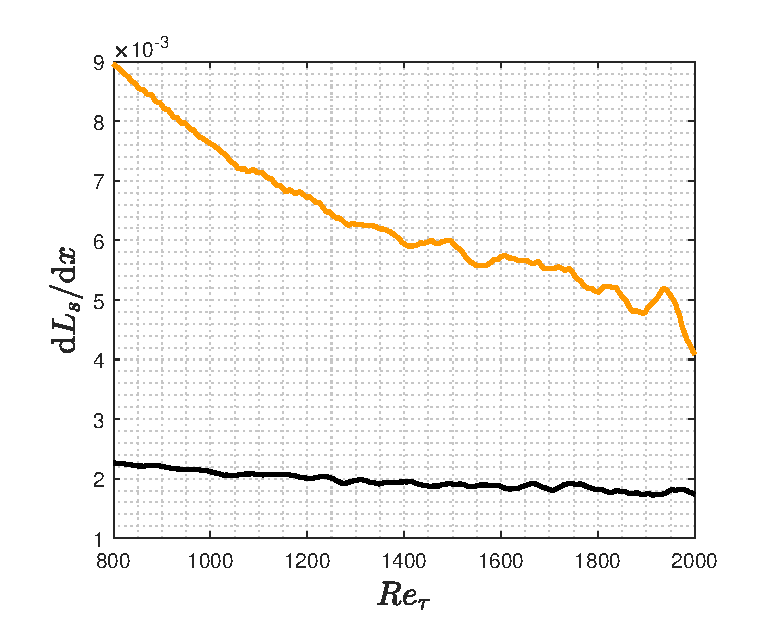
\includegraphics[width=0.49\textwidth]{fig7c.eps}
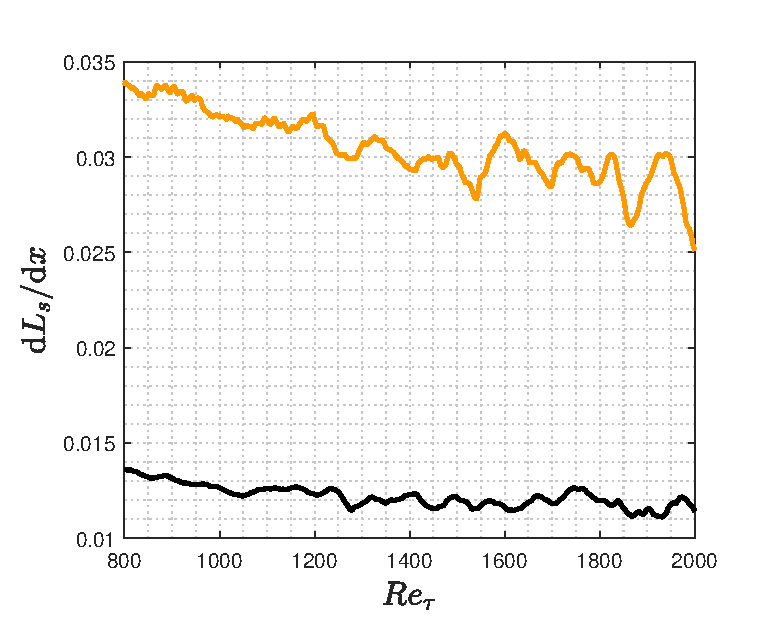
\includegraphics[width=0.49\textwidth]{fig7d.eps}
\caption{Different pressure-gradient parameters based on the self-similarity analysis for the outer layer performed in \citet{Gibis2019}. Left column represents the edge scaling, where $L_s=\delta^*$ and $U_s=U_e$. Right column shows the Zagarola--Smits scaling with $L_s=\delta_{99}$ and $U_s=U_{e}\delta^*/\delta_{99}$. A Savitzky--Golay filter has been applied to $\textrm{d} L_s/\textrm{d}x$ as in \cite{Gibis2019}. The black solid line represents the ZPG by \cite{E-AmorZPG} and the orange line is the present b1.4 simulation.}
\label{fig:pg_parameters}
\end{figure}

\begin{figure} 
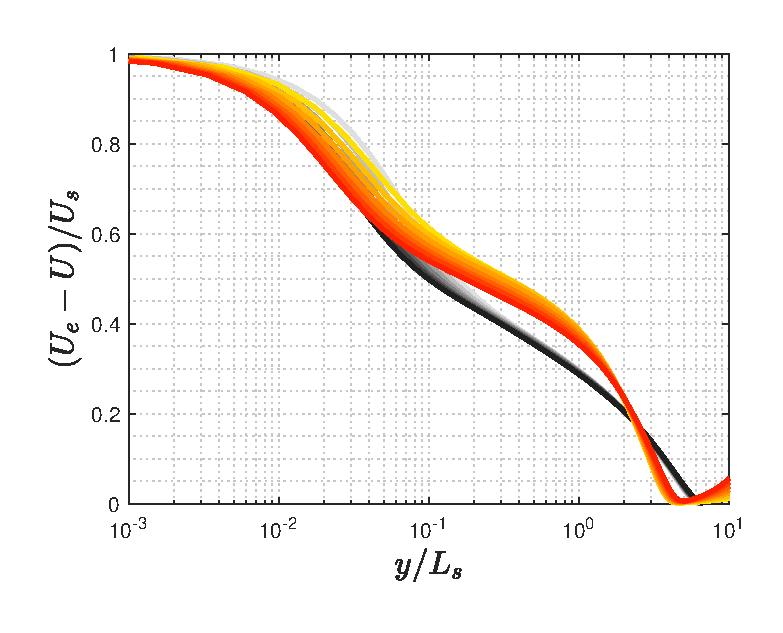
\includegraphics[width=0.49\textwidth]{fig8a.eps}
\includegraphics[width=0.49\textwidth]{fig8b.eps}
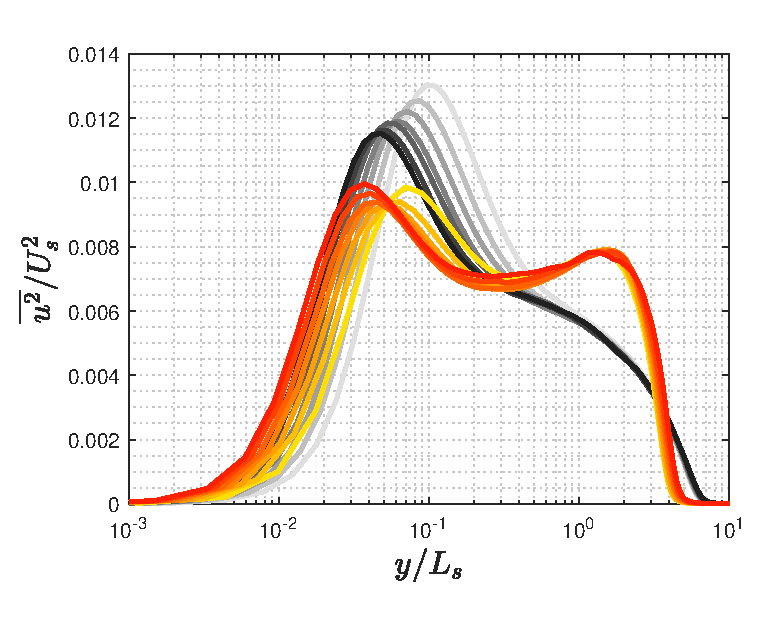
\includegraphics[width=0.49\textwidth]{fig8c.eps}
\includegraphics[width=0.49\textwidth]{fig8d.eps}
\caption{(Top) Mean velocity defect and (bottom) streamwise Reynolds stress scaled with: edge (left) and Zagarola--Smits (right) scalings. Profiles from $Re_{\tau}=800$ to $Re_{\tau}=2000$. Lines in gray scale represent ZPG data \citep{E-AmorZPG}, increasing the Reynolds number from white to black. APG data from the b1.4 simulation increases Reynolds number from yellow to red.}
\label{fig:def_U_uu}
\end{figure}

In figure \ref{fig:def_U_uu} we use the edge and ZS scalings for the streamwise mean velocity defect and the streamwise RS for the profiles within the ROI.
The first observation is the common good agreement of both scalings from the logarithmic region all the way to the edge of the TBL in the ZPG.

Equation~(\ref{eq:defect_scaled_2}) shows the definition of $\delta^*$. For the ZS and edge scalings, the velocity and length scales are just a combination of the parameters present in equation~(\ref{eq:defect_scaled_2}) ($U_e$, $\delta^*$, $\delta_{99}$), therefore we can divide both sides by the term $U_e \delta^*$ and using the length and velocity scales in table \ref{tab:Scaling_parameters} it is possible to rewrite the integral in a common form (right-hand side of equation~(\ref{eq:defect_scaled_2})) for both ZS and edge scalings.

\begin{equation}\label{eq:defect_scaled_2}
    \int_{0}^{\delta_{99}} (U_e-U) \textrm{d} y = U_e \delta^*  \Rightarrow \int_{0}^{\delta_{99}/L_s} \frac{U_e-U}{U_s} \textrm{d}(y/L_s)=1. 
\end{equation}

Using this form we can directly relate the integral with the mean defect velocity curves in figure \ref{fig:def_U_uu}. 
 The value of the normalized integral of the mean velocity defect is the same for both scalings, where the integrands are the various curves and the only difference would be the upper limit of the integration. That upper limit in the ZS scaling does not change with the Reynolds number: it is 1 since $L_s=\delta_{99}$. The upper limit for the edge scaling is variable with Reynolds number because $L_s=\delta^*$. 
The functional form in the edge scaling fixes all the profiles to start from the same point, thus the differences between profiles increase from the wall. The functional form of the ZS scaling makes the profiles start from different values for each Reynolds number, and since the value of the integral is the same and the upper limit is also the same for all profiles, the differences are concentrated close to the wall, allowing for a better collapse in the outer region of the TBL.
This can be observed in figure \ref{fig:def_U_uu} (top right), where the ZS scaling exhibits a better collapse even in the overlap region. 
The edge scaling, figure \ref{fig:def_U_uu} (top left), exhibits a good collapse in the wake region, with differences in the overlap region.


We have previously discussed that the inner peak of $\overline{u^2}$ has a location $y^+ \simeq 15$. As shown in figure \ref{fig:def_U_uu} (bottom), and also in figure \ref{fig:uupeaks_loc}b) and c), the outer-peak location for the edge scaling is at $y/\delta^*=1.4$ and around $y/\delta_{99}=0.35$ for the ZS scaling.
While there is a better collapse in the outer region of the mean defect profiles using the ZS scaling, the $\overline{u^2}$ profiles collapse in the outer region when using the edge scaling.
Our results suggests that it is not possible to collapse the wall-normal profiles at all positions 
with a single length scale. In the mean flow, the inner region collapses in inner scaling and the outer region using the ZS scaling. Regarding the streamwise RS, the location of the near-wall peak slightly varies around $y^+\simeq 15$, it slowly grows with the Reynolds number and the slope is larger with higher $\beta$, whereas both the magnitude and location of the outer peak are fixed using the edge scaling. 
Since the inner and outer scales are related by $\Rey_{\tau}$, to achieve self-similarity throughout the whole profile would require that $\Rey_{\tau}$ remains constant in $x$, which is not the case even in the ZPG. 

\begin{figure}
\includegraphics[width=0.49\textwidth]{fig9a.eps}
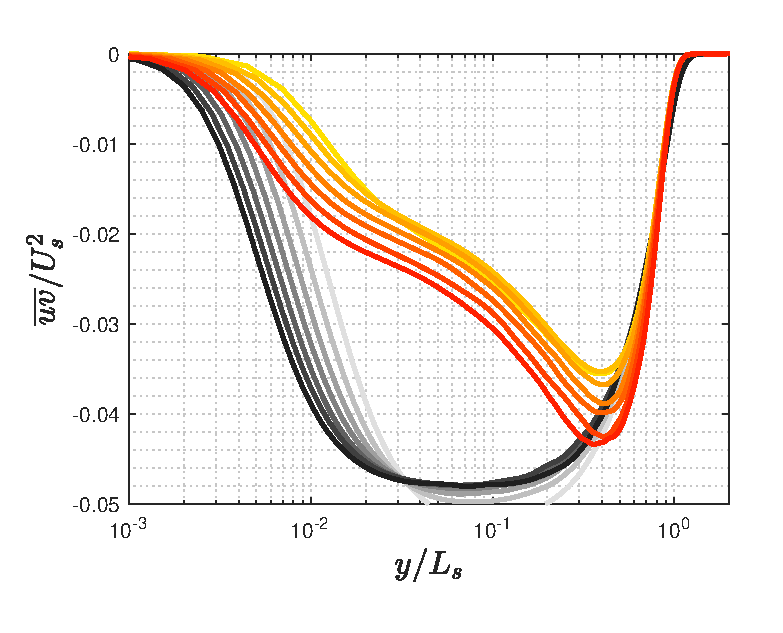
\includegraphics[width=0.49\textwidth]{fig9b.eps}
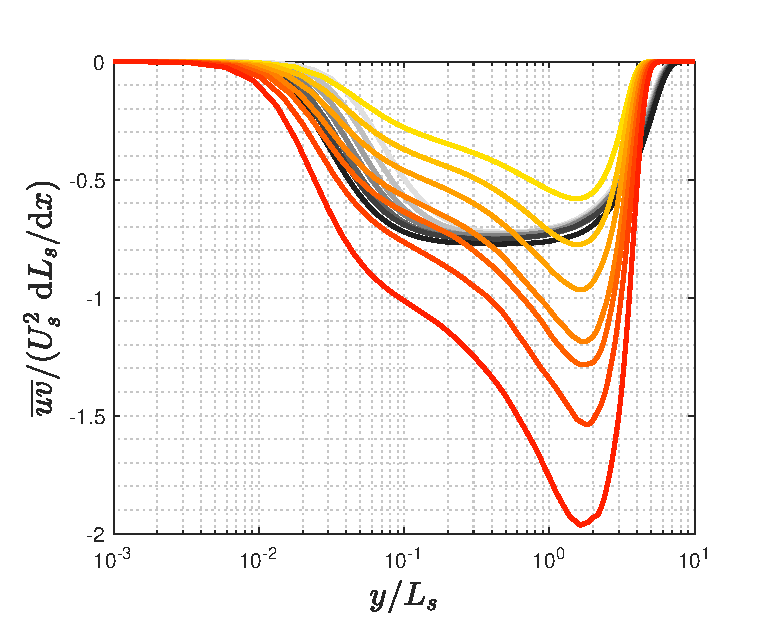
\includegraphics[width=0.49\textwidth]{fig9c.eps}
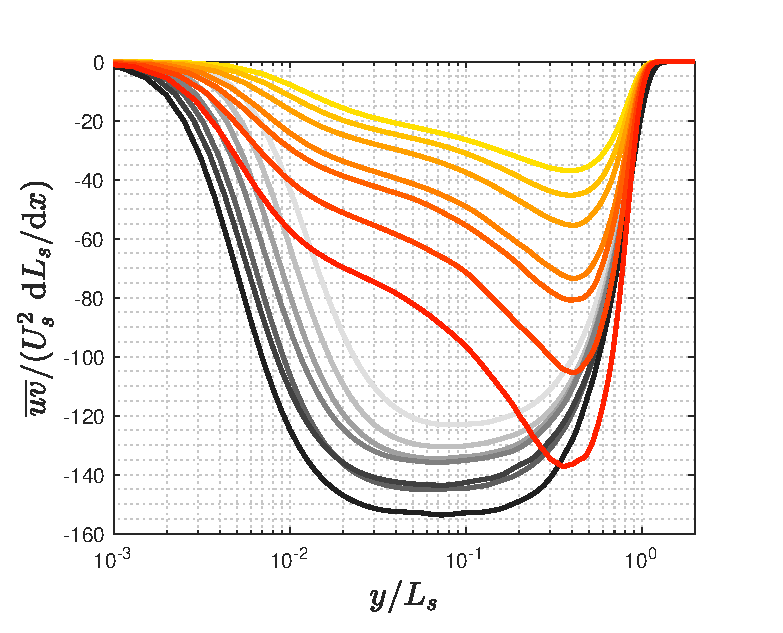
\includegraphics[width=0.49\textwidth]{fig9d.eps}
\caption{Reynolds shear stress $\overline{uv}$ scaled with: edge (left) and Zagarola--Smits (right) scalings. The second row shows the effect of the evolution of the characteristic length scale $\textrm{d} L_s/\textrm{d}x$. Profiles from $Re_{\tau}=800$ to $Re_{\tau}=2000$. Lines in gray scale represent ZPG data \citep{E-AmorZPG}, increasing the Reynolds number from white to black. APG data from the b1.4 simulation increases Reynolds number from yellow to red.}
\label{fig:uv_scalings}
\end{figure}

In the next similarity analysis we consider the Reynolds shear stress, where in figure \ref{fig:uv_scalings} (top) we consider $U_s^2$, and in figure \ref{fig:uv_scalings} (bottom) we use $U_s^2 \textrm{d} L_s/\textrm{d}x$ as in \cite{Kitsios2016, Gibis2019}.
The edge scaling leads to a moderate collapse of the $\overline{uv}$ profiles in the outer region, although the collapse is not as good as the one observed for $\overline{u^2}$.
The additional term $\textrm{d} L_s/\textrm{d}x$ applied to the Reynolds shear stress, worsens the collapse for the APG in both scalings, while it improves the collapse for the ZPG in the edge scaling.

To summarize, the edge scaling yields a good scaling of the APG profiles in the outer region, and given the good collapse with viscous units close to the wall, it can be stated that the APG TBL is in near-equilibrium  \citep{Marusic_PoF_2010, bobke2017} conditions in the ROI.
The ZS scaling leads to a better collapse in the outer region of the mean defect profiles.

As observed in figure \ref{fig:kitsios_scalings},
comparing the first three profiles for both the ZPG and b1.4 cases a clear lack of collapse 
can be observed, and as discussed in figure \ref{fig:def_U_uu} the profiles only collapse in the inner or outer regions using the adequate scaling. We argue that any claims of self-similarity throughout the complete boundary layer may be based on limited regions of near-equilibrium conditions, which may hide the existing Reynolds-number trends. 
With these considerations we remark the importance of considering long regions of near equilibrium, where it is possible to clearly observe the trends in the inner and outer layers and to assess how the scales separate as the TBL develops. 

\begin{figure}
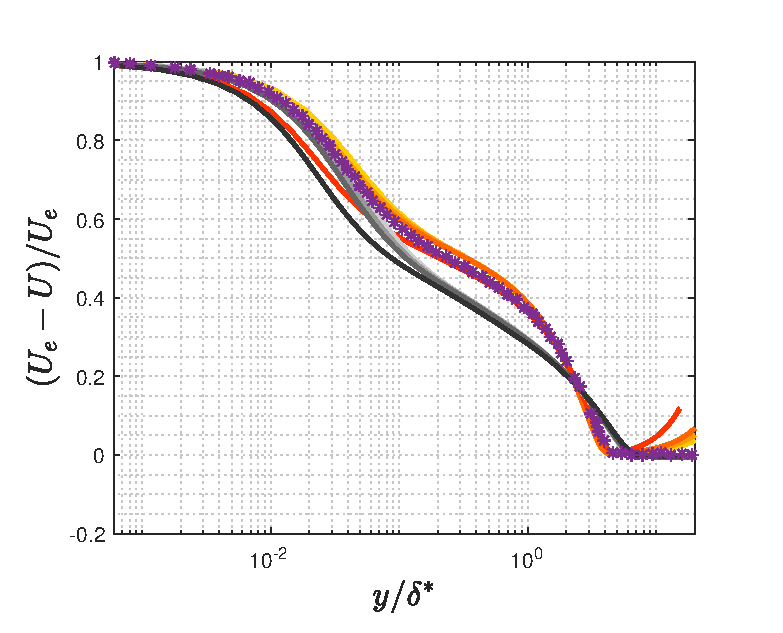
\includegraphics[width=0.32\textwidth]{fig10a.eps}
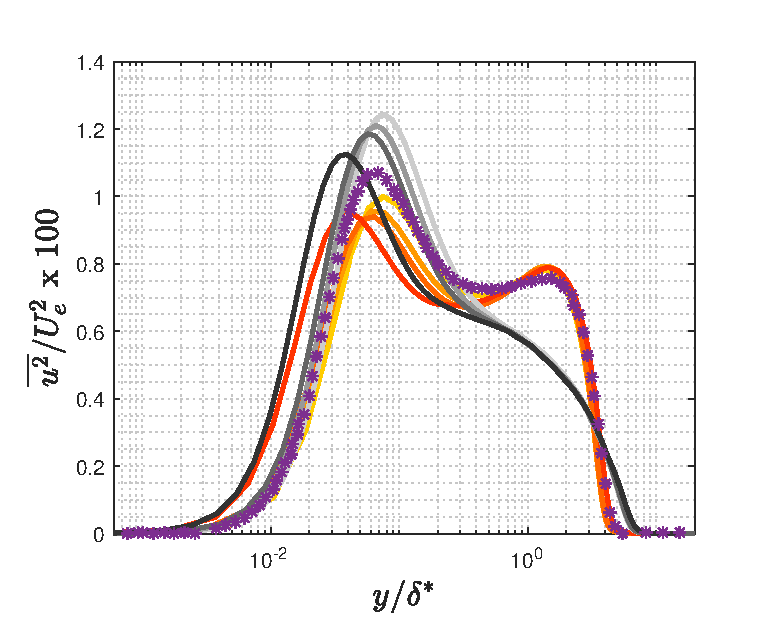
\includegraphics[width=0.32\textwidth]{fig10b.eps}
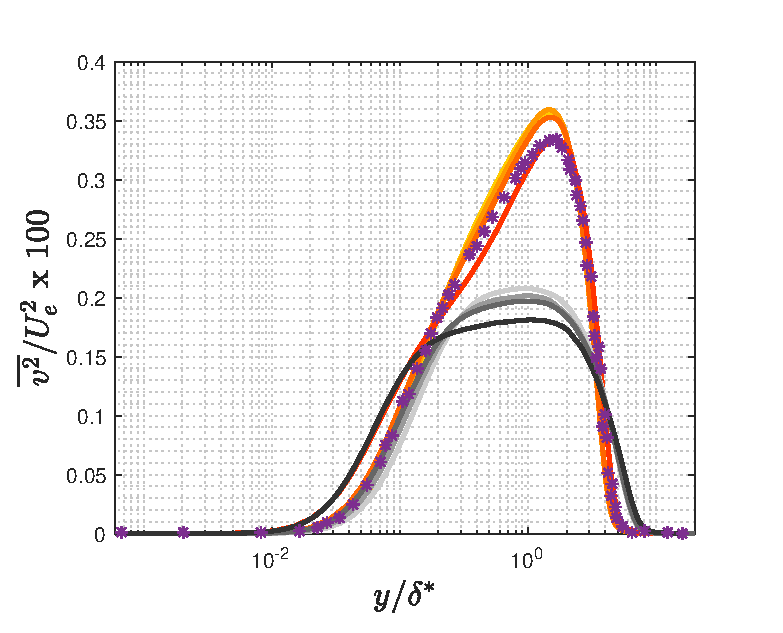
\includegraphics[width=0.32\textwidth]{fig10c.eps}
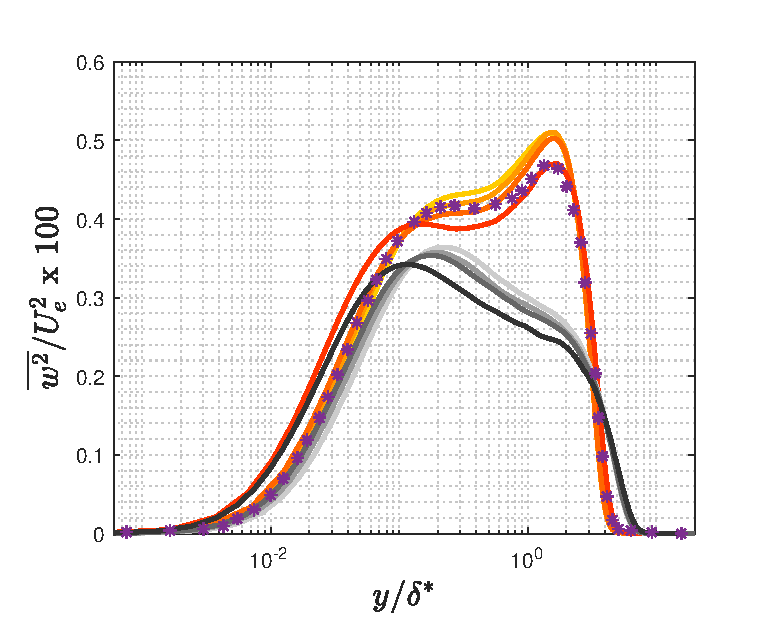
\includegraphics[width=0.32\textwidth]{fig10d.eps}
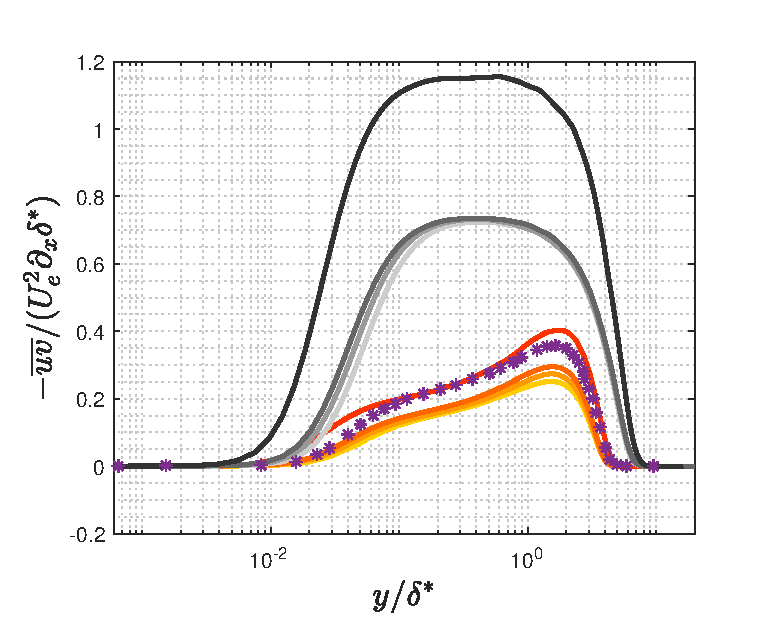
\includegraphics[width=0.32\textwidth]{fig10e.eps}
\caption{Mean streamwise velocity defect and Reynolds-stress tensor components $\overline{u^2}$, $\overline{v^2}$, $\overline{w^2}$, $\overline{uv}$ scaled using the edge scaling as in \cite{Kitsios2016}, and using the streamwise derivative of the length scale $\partial_x \delta^*$ in the case of $\overline{uv}$. The purple asterisks are used for the collapsed data by \cite{Kitsios2016}. The profiles have been taken at $\Rey_{\theta}=\{3500, 4150, 4800, 8200\}$, where the first three are in the same range as \cite{Kitsios2016} and the last at one is the highest $\Rey_{\theta}$ available in ZPG and b1.4 cases. Gray lines show the ZPG data growing in $\Rey$ from light to dark. The b1.4 lines show increase in Reynolds number from yellow to red.}
\label{fig:kitsios_scalings}
\end{figure}


